% !TEX root =  main.tex



\chapter{Background Knowledge}
\label{chap:background}
\pagestyle{plain}

In this chapter, we give context on the terminologies, definitions and algorithms employed in our system.

\section{Schema Matching}\label{schemaMatching}
Schema matching is the task of finding semantic correspondence between two schemas, where a schema is defined as a set of elements connected by some structure \cite{schemaMatching}. It plays a critical role in data integration and translation applications. An use case example is the integration of a real estate schema and a property tax schema, where each schema may have structural and terminological differences, but occur in the same real-world domain and thus can be unified under the same schema. In the case of relational data, schema matching techniques can be used to determine the joinability and unionability between attributes of two tables \cite{valentine}. Schema matching techniques for relational data work on attributes/columns of tables and can be roughly classified into two categories: schema-based and instance-based:

\begin{description}
    \item[Schema-based] These types of matchers only consider the schema-level information of a dataset such as table name, attribute names, description, data type, constraints, etc \cite{cupid}. The similarity of the information can be calculated by e.g. how much the attribute name syntactically or semantically overlap, is the data type similar (short and int or text and varchar).
    \item[Instance-based] When schema-level information is limited, the instances of an attribute can provide correct interpretation of schema information. Examples include the similarity in how the instances of two attributes overlap, or how the format patterns look like (money-related instances contain a currency symbol, whereas a zip code does not).
\end{description}

Matching process usually involves calculating the degree of similarity by a normalized numeric value in the range 0 to 1. It is also possible to combine different matching techniques together, then an algorithm is applied to aggregate the score of different techniques to one single score that is used to rank the results \cite{coma}. In our implementation, we will follow this hybrid strategy.

\section{Similarity Metrics}

\subsection{Levenshtein distance similarity}

In order to capture the syntactic relatedness between two words \(s\) and \(t\), we use the Levenshtein edit distance. The Levenshtein distance between two words is the minimum required number of insertions, deletions or substitutions of a character to transform one word into another \cite{levenshtein}. Since this metric measures distance, we convert it into a similarity metric by dividing the distance with the length of the longest word, normalizing it to the range 0 and 1, and then subtract it from 1 to get a similarity score:

\[sim_{levenshtein} = 1 - \frac{dist(s, t)}{max(s, t)}\]

\subsection{WordNet Similarity}\label{wordnet}

In order to capture the semantic relatedness between two words, we use the machine-readable lexical database WordNet \cite{wordnet}, which contains English words grouped into sets of synonyms (synsets) and structured in a hierarchical is-a relation. One algorithm that can be used to calculate the similarity of two words \(s\) and \(t\) is the Wu-Palmer algorithm \cite{wuPalmer}, which considers the depths of two synsets in the Wordnet hierarchy as well as the depth of the least common subsumer (LCS) i.e. the most specific concept that is the ancestor of both \(s\) and \(t\):

\[sim_{wordnet}(s, t) = 2 \cdot \frac{depth(LCS)}{(depth(s) + depth(t))}\]

To extend the similarity of two words to two sets of words / sentences \(q_i\) and \(q_j\), we use an equation similar to ones from \cite{wordnetSim} and \cite{cupid}:

\[score(q_i, q_j) = \frac{\Sigma_{s \in q_i} sim_m(s, q_j) +\Sigma_{s \in q_j} sim_m(s, q_i)}{|q_i| + |q_j|}\]

where \(sim_m(s, q_j\) is the similarity score of s and the word in \(q_j\) that has the highest similarity score. If a word does not exist in the dictionary, we fall back to Levenshtein distance similarity for the calculation.

\subsection{Jaccard Similarity}\label{js}

The Jaccard similarity/coefficient is a metric used to calculate the similarity of two sets  \cite{miningOfMassiveDatasets}. Given two sets \(A\) and \(B\), the Jaccard coefficient \(J(A, B)\) of the two sets is defined by the ratio between the size of the intersection to the size of the union:

\[
J(A, B) = \frac{|A \cap B|}{|A \cup B|}
\]

For example, if \(A = \{1, 2, 3\}\) and \(B = \{2, 3, 5\}\), then \(J(A, B) = \frac{1}{2}\). The value of Jaccard coefficient ranges from 0 to 1. In \cite{tusZhu}, the authors show that a high Jaccard coefficient value between sets suggests a high probability that the elements of the sets are drawn from the same domain. Therefore, we can utilize this measure to find unionable columns for a given column of a dataset.

\subsection{Set Containment}\label{jc}

One problem with Jaccard coefficient is that the measure is symmetric. In the case where sets are of vastly different sizes, the measure is biased to sets with smaller sizes \cite{lshEnsemble}. For example, consider the query set:

\begin{itemize}
    \item \(Query\) = \{Ontario, Toronto\}
\end{itemize}

and the two sets:

\begin{itemize}
    \item \(Provinces\) = \{Alberta, Ontario, Manitoba\}
    \item \(Locations\) = \{Illinois, Chicago, New York City, New York, Nova Scotia, Halifax, California, San Francisco, Seattle, Washington, Ontario, Toronto\}
\end{itemize}

We see that while the \(Locations\) set contain all the elements of the \(Query\) set, their Jaccard similarity is only 0.083, while the similarity between \(Query\) and \(Provinces\) is at 0.25, indicating a higher degree of relatedness despite \(Provinces\) containing only one similar element with \(Query\). Due to this reason, there is another asymmetric measure used in the literature for comparing set similarity called set containment.

Given two sets \(A\) and \(B\), the set containment of \(A\) in \(B\) is defined as:

\[
J_C(A, B) = \frac{|A \cap B|}{|A|}
\]

and vice versa for the containment of \(B\) in \(A\):

\[
J_C(B, A) = \frac{|A \cap B|}{|B|}
\]

Using set containment, we see that \(J_C(Q, Provinces)\) is 0.5, while \(J_C(Q, Locations)\) is now 1.0. This measure is proven to be useful in identifying primary-key/foreign-key relationships, which enables the process of finding joinable datasets \cite{lazo}.

\section{Q-gram}

Another way to measure the syntactic relatedness of two words beside using Levenshtein distance similarity, is by comparing their q-grams sets. A q-gram (or n-gram) of a string is simply a substring of length q \cite{qgram}. The set of q-grams of a string is then constructed by finding all q-grams within that string. We utilize the Jaccard coefficient mentioned above to calculate the similarity of the q-grams sets. For example, to compare "house" and "horse" with a q value of 2:

\begin{itemize}
    \item 2-grams of "house": \(s = \{ho, ou, us, se\}\)
    \item 2-grams of "horse": \(t = \{ho, or, rs, se\}\), therefore:
\end{itemize}

\[sim_{qgram}(house, horse) = J(s,t) = \frac{1}{3}\]

The advantage of this measure compared to Levenshtein distance similarity is, they can be efficiently calculated using locality sensitive hashing, which is explained in section \ref{lsh}.

\section{MinHash Sketch}

When a set size goes to the degree of thousands of elements or higher, calculating the Jaccard coefficient/containment of two sets can become computationally very expensive. Instead, we transform the sets into smaller, fixed-size representations called "sketches" and calculate the similarity measures using only these sketches \cite{miningOfMassiveDatasets}. One of these types of sketches is called MinHash.

The core idea behind MinHash is to apply a hash function to the elements of a set, simulating a random permutation, and then store the minimum hash value observed. By doing this multiple times with different hash functions, we create a set of minimum values that serves as a compact representation of the original set. The interesting property of MinHash is that, the probability of 2 sets having the same minimum hash value when applied the same hash function is directly related to the Jaccard coefficient between two sets:

\[Pr[h_{min}(A) = h_{min}(B)] = \frac{|A \cap B|}{|A \cup B|} = J(A, B)\]

Thus, by using \(k\) multiple hash functions, the Jaccard coefficient can be estimated as:

\[J(A, B) = \frac{1}{k} \cdot \Sigma \; \mathbf{1}((h^i_{min}(A) = h^i_{min}(B))\]

Where the function \(\mathbf{1}\) returns 1 if the condition inside the argument is true and 0 otherwise.

\section{Locality Sensitive Hashing} \label{lsh}

While MinHash allows us to efficiently calculate similarity of sets, it remains a challenge to find the pairs with greatest similarity among large collection of sets, since we would need to perform up to pairwise calculations of all pairs of sets to get the correct result. However, for our task we would want only the most similar pairs or pairs that are above some similarity threshold. Therefore, we accept a slight loss in accuracy and use approximate methods to focus our attention only on pairs that are likely to be similar, without investigating every pair. One such method is locality sensitive hashing (LSH), which is widely used in data discovery tasks due to its exploratory and imprecise nature. \cite{miningOfMassiveDatasets, lazo}

The general idea of LSH is to use a locality sensitive hash function to hash items into buckets, where the amount of buckets is significantly smaller than the universe of the possible input items. Locality sensitive hash functions are functions which map inputs that are similar to the same hash value with high probability, while minimizing that probability for inputs that are dissimilar \cite{lshDefinition}. If we use these hash functions to map elements in the buckets, similar items would fall into the same buckets with high probability. Thus, in order to find similar items with our input, we need only to check the similarity of the items in the bucket that our input falls into. 

In literature, the way a MinHash sketch in hashed into a LSH index is by first diving it into \(b\) bands of equal length, then hash each of these bands into individual bucket array. Two sketches are similar if in any band, there is a bucket collision ( figure \ref{fig:lsh}). The use of LSH functions mean the more similar two sketches are, the higher the probability they will be identical in at least one band, making them candidate pairs. This banding strategy thus enhances the likelihood of detecting similar columns while minimizing accidental collisions for dissimilar pairs.

\begin{figure}[h]
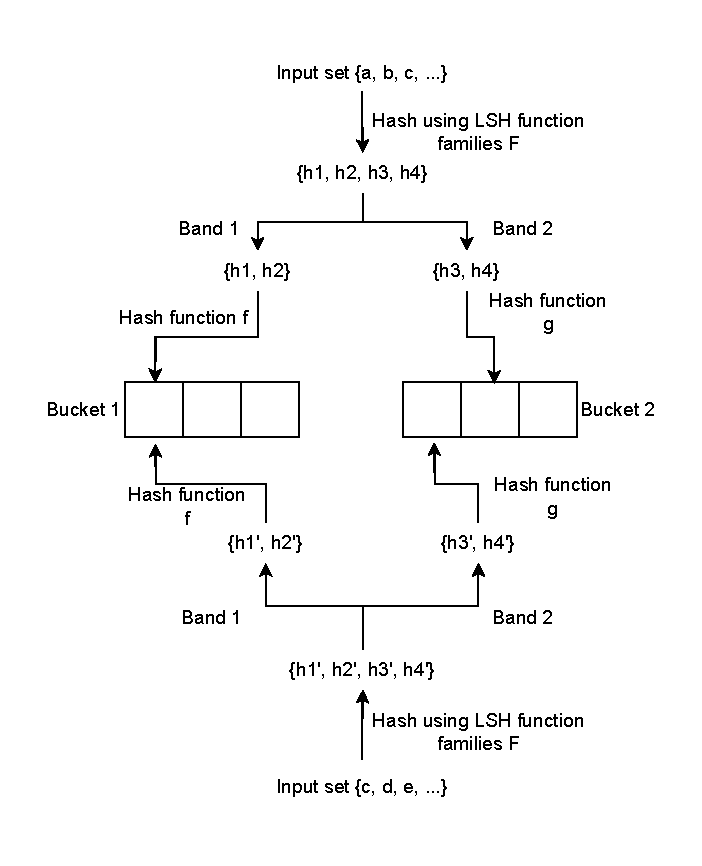
\includegraphics[scale=0.8]{lsh.pdf}
\centering
\caption{Example of the LSH banding technique. The two sketches collide in bucket 1, hence a match}
\label{fig:lsh}
\end{figure}

\section{REST API}

Representational State Transfer (REST) is a term coined by Fielder in his PhD dissertation \cite{rest}. It is a software architectural style that defines a set of constraints on how the components of a distributed hypermedia system like in Web should communicate with each other. Rest API is an application programming interface (API) that adheres to the constraints of REST architectural style. While there are six constraints that Fielder introduced in his work, the three most important constraints for our work are:

\begin{itemize}
    \item \textbf{Uniform interface}: REST components communicate with each other via representation or abstraction of resources but still need to contain enough information to manipulate the underlying resources. They are identifiable using Unique Resource Identifiers (URIs).
    \item \textbf{Client-server decoupling}: Client and server are independent of each other. Communications between client and server happen between an interface, i.e. the URI of a resource.
    \item \textbf{Statelessness}: Each request from client to server must contain all the information required to process the request, without utilizing additional server context.
\end{itemize}

Overall, these constraints allow a system to have better performance thanks to its flexibility and scalability. In practice, REST APIs work through HTTP connections, which fit the constraints of REST perfectly. A REST API request contains the following component:

\begin{itemize}
    \item \textbf{Endpoint}: The URI where the requested resource can be retrieved. For instance, the URI for a HTTP request is an Unified Resource Locator (URL): \nolinkurl{https://song.com/trackID/1}
    \item \textbf{Method}: The HTTP method that is used to operate on the resources. The common methods are GET (retrieve a resource), POST (Create a new resource), PUT (update existing resource) and DELETE (remove a resource).
    \item \textbf{Headers}: Provide metadata-level information about the request like the content type or its encoding.
    \item \textbf{Parameters}: Additional information that is appended to the URL to specify server's action in a more detailed way.
    \item \textbf{Request body}: The data, which is a representation of resource that is sent to the server. It is often formatted in JSON.
\end{itemize}

Upon receiving a request, the server responds with a HTTP response, containing the response metadata, a status code to indicate whether the request was successful or not and the resource representation itself in the body. Due to the nature of our system working in a distributed environment, REST APIs are employed to facilitate communication between the components.